\documentclass[../../DS]{subfiles}

\begin{document}
\begin{sloppy}
    
\section{图}

    \textbf{基本定义} \\
    数学定义: 图$G$由顶点$V$和边$E$组成, 记为$G=(V, E)$. $V(G)$表示$G$中顶点的非空子集, $E(G)$表示$G$的边. $V = \{v_1, v_2, \dots\}$, $E = \{(u, v) | u \in V, v \in V\}$. \textbf{图的顶点数(图的阶数)}: $|V|$, \textbf{图的边数}: $|E|$ \\
    图不可以是空图, 图\textbf{至少有一个结点}. 顶点集$V$一定非空, 边集\textbf{可以为空} \\
    \textbf{弧}: 有向边, 顶点的有序对, 记为$<v, w>$, $v \to w$, \textbf{弧尾}: $v$, \textbf{弧头}: $w$. 称: $<v, w>$为v到w的弧, 或$v$ 邻接\textbf{到} $w$ \\
    \textbf{边}: 无向边. 记为$(v, w)$或者$(w, v)$. $v, w$互为 \textbf{邻接点}, 称: 边$(v, w)$依附于w和v, 或者边$(v, w)$与$v, w$相关联 \\
    \textbf{简单图(存在有向无向之分)}: 1. 不存在重复边; 2. 不允许顶点到自身的边 \\
    \textbf{复杂图}: 存在重复边或者存在顶点到自身的边 \\
    \textbf{顶点的度}: \\
    \textbf{无向图}: 顶点$v$的度是依附于$v$的边的数量, 记为$TD(v)$. \textbf{无向图}全部顶点的度之和为边数的2倍(一条边连接两个顶点), 即$\sum\limits_{i=1}^{n}TD(v_i) = 2 |E|$ \\
    \textbf{有向图}: 区分\textbf{入度}, \textbf{出度}, \textbf{度}. \\
    \textbf{入度}: 以$v$为终点的边的数量, 记作$ID(v)$. \textbf{出度}: 以$v$为起点的边的数量, 记作$OD(v)$. \\
    \textbf{度}: 入度与出度之和, 记作$TD(v) = ID(v) + OD(v)$. 有向图中: $\sum\limits_{i=1}^{n}ID(v_i) = \sum\limits_{i=1}^{n}OD(v_i) = |E|$ \\
    \textbf{路径}: 顶点$v_p$到$v_q$之间的序列$v_p, v_1, v_2, \dots, v_q$ \\
    \textbf{路径长度}: 路径上边的数目 \\
    \textbf{回路(环)}: 首末顶点相同的路径. 若一个图有$n$个顶点, 有多于$n-1$条边, 则该图\textbf{一定有环} \\
    \textbf{简单路径}: 顶点不重复出现的路径 \\
    \textbf{简单回路}: 除了首末顶点之外, 其他顶点不重复出现的回路 \\
    \textbf{距离(区分有向无向)}: 从$u$\textbf{到}$v$的\textbf{最短}路径长度. 若$u, v$之间不存在路径, 则距离为无穷$\infty$ \\
    \textbf{子图}: 若$G = (V, E), G' = (V', E')$, $V'$是$V$的子集, $E'$是$E$的子集, 则$G'$是$G$的子图. 若要构成子图, 则$E'$涉及的顶点必须全在$V'$中, 否则不构成图, 因此, 不是VE的任何子集都能构成G的子图 \\
    \textbf{生成图}: $G'$是$G$的子图, 且$V(G') = V(G)$, 即子图包含原图的全部顶点 \\
    \textbf{连通}: \textbf{无向图中}, 顶点v和w之间存在\textbf{路径}. \\
    \textbf{连通图}: 无向图中任意两个顶点都是连通的; \textbf{非连通图}: 不是连通图的无向图. \textbf{极大连通子图(连通分量)}: 1. 连通图; 2. 包含尽可能多的顶点和边(\textbf{不能被任何另外一个连通子图所包含}) \\
    对于有$n$个顶点的无向图, 若为\textbf{连通图}, \textbf{最少有} n-1条边(一个顶点连接所有); 若保证为\textbf{非连通图}, \textbf{最多有} $\binom{n-1}{2}$条边(n-1个顶点两两相连, 孤立一个顶点) \\
    \textbf{强连通}: \textbf{有向图}中, 对于顶点v, w, 从v到w和从w到v的路径都存在(不一定有$<v, w>$或$<w, v>$), 则称这两个顶点强连通 \\
    \textbf{强连通图}: 有向图中, 任意两个顶点都是强连通的 \\
    \textbf{强连通分量}: 1. 强连通图; 2. 包含尽可能多的顶点和边. 若一个图是强连通图, \textbf{最少有}n条边(构成环) \\
    \textbf{生成树}: \textbf{连通图}中包含图中全部顶点的一个\textbf{极小连通子图}. 1. 包含全部顶点; 2. 边尽可能少. n个顶点的图, 其生成树只能有n-1条边. 生成树可能有多个 \\
    \textbf{生成森林}: \textbf{非连通图}中, 连通分量的生成树构成非连通图的生成森林 \\
    \textbf{边的权值}: 每条边都可以标注的有意义的数值 \\
    \textbf{网(带权图)}: 边有权值的图 \\
    \textbf{带权路径长度}: 路径上所有边的权值之和
    
    \newpage
    \noindent
    \textbf{完全图(简单完全图)}: 对于n个顶点的\textbf{无向图}, 有$\binom{n}{2} =  \frac{n(n-1)}{2}$条边的图(任意两个顶点之间有边); 对于n个顶点的\textbf{有向图}, 有$2 \binom{n}{2} = n(n-1)$条边的图(任意两个顶点之间有方向相反的两条边). n个顶点, 无向图, 边的条数$\in[0, \binom{n}{2}]$; 有向图, 边的条数$[0, n(n-1)]$ \\
    \textbf{稠密图}: 边很多的图; \textbf{稀疏图}: 边很少的图. 一般, 满足$|E| < |V| \log_2 |V|$ 或 $|E| \ll \frac{|V|(|V|-1)}{2}$可视为稀疏图(没有绝对的判断标准) \\
    \textbf{有向树}: 一个顶点的入度为0, 其余顶点的入度均为1的有向图(不是强连通图) \\
    \textbf{树}: 1. 无向图; 2. 不存在回路; 3. 连通; 

    \begin{figure}[htbp]
        \centering
        \includegraphics[width=0.5\columnwidth]{./graphconnect.png}
    \end{figure}

    \textbf{找强连通分量} \\
    1. 不断分离出孤立顶点 \\
    2. 不断分离出没有出度的顶点和与其相连的边 \\
    3. 不断分离出没有入度的顶点和与其相连的边

    \begin{figure}[htbp]
        \centering
        \begin{subfigure}{0.45\textwidth}
            \begin{tikzpicture}[node distance=1.5cm, , >=Stealth]
                \tikzstyle{vertex}=[circle, draw, minimum size=0.5cm]
            
                \node[vertex] (A) {A};
                \node[vertex, below right of=A] (D) {D};
                \node[vertex, above right of=D] (C) {C};
                \node[vertex, below left of=D] (B) {B};
                \node[vertex, below right of=D] (E) {E};
                \node[vertex, below left of=A] (F) {F};
                \node[vertex, below right of=C] (G) {G};
                
                \draw[->] (A) to[bend left=20] (C);
                \draw[->] (C) to[bend left=20] (A);
                \draw[->] (B) -- (A);
                \draw[->] (D) -- (A);
                \draw[->] (C) -- (D);
                \draw[->] (D) -- (E);
                \draw[->] (E) -- (C);
                \draw[->] (B) -- (D);
                \draw[->] (B) -- (E);
                \draw[->] (C) -- (G);
                \draw[->] (E) -- (G);
            \end{tikzpicture}
            \caption{有向图}
        \end{subfigure}
        \begin{subfigure}{0.45\textwidth}
            \begin{tikzpicture}[node distance=1.5cm, , >=Stealth]
                \tikzstyle{vertex}=[circle, draw, minimum size=0.5cm]
                
                \node[vertex] (A) {A};
                \node[vertex, below right of=A] (D) {D};
                \node[vertex, above right of=D] (C) {C};
                \node[vertex, below right of=D] (E) {E};
                \node[vertex, below left of=A] (F) {F};
                \node[vertex, below right of=C] (G) {G};
                \node[vertex, right of=G] (B) {B};

                \draw[->] (A) to[bend left=20] (C);
                \draw[->] (C) to[bend left=20] (A);
                \draw[->] (D) -- (A);
                \draw[->] (C) -- (D);
                \draw[->] (D) -- (E);
                \draw[->] (E) -- (C);
            \end{tikzpicture}
            \caption{4个强连通分量}
        \end{subfigure}
    \end{figure}

\subsection{图的存储}

\subsubsection{邻接矩阵法}

    顺序存储. 用一个一维数组存储图中顶点的信息, 用一个二维数组存储图中边的信息, 其中, 二维数组称为\textbf{邻接矩阵}. 在简单应用中, 可以忽略一维数组, 不存储顶点信息. 邻接矩阵的空间复杂度为$O(|V|^2)$. \textbf{稠密图}适合使用邻接矩阵 
    图中, 顶点自身与自身不认为有边连接. 记有n个顶点的图之顶点为$v_1, v_2, \dots, v_n$

    \textbf{非带权图}
    
    % new two columns
    \vspace{-2\baselineskip}
    \begin{center}
    \begin{minipage}[t]{0.48\textwidth}
    \vspace{0pt}
    \begin{center}
        $
        A[i][j] = \begin{cases}
            1, <v_i, v_j>\mbox{或}(v_i, v_j)\mbox{是图中的边} \\
            0, <v_i, v_j>\mbox{或}(v_i, v_j)\mbox{不是图中的边} \\
        \end{cases}
        $
    \end{center}
    \end{minipage}
    \begin{minipage}[t]{0.48\textwidth}
    \vspace{0pt}
        注意i, j的先后关系在有向图中不可以对换. \textbf{有向图}中 \verb|A[i][j]|是边 \verb|i->j|. \textbf{无向图}中, 邻接矩阵是一个\textbf{唯一的}对称矩阵(上下三角压缩存储)
    \end{minipage}
    \end{center}

    \vspace{-1\baselineskip}
    \textbf{带权图}

    % new two columns
    \vspace{-2\baselineskip}
    \begin{center}
    \begin{minipage}[t]{0.53\textwidth}
    \vspace{0pt}
    \begin{center}
        $
        A[i][j] = \begin{cases}
            w_{ij}, <v_i, v_j>\mbox{或}(v_i, v_j)\mbox{是图中的边} \\
            0 \mbox{或} \infty, <v_i, v_j>\mbox{或}(v_i, v_j)\mbox{不是图中的边} \\
        \end{cases}
        $
    \end{center}
    \end{minipage}
    \begin{minipage}[t]{0.45\textwidth}
    \vspace{0pt}
        1. $\infty$可以定义为 \verb|MAXINT|; 2. 部分情况下, 自身与自身(对角线): 0, 无边: $\infty$
    \end{minipage}
    \end{center}

    \newpage
    \textbf{数据结构}
    \begin{lstlisting}[style = Cpp]
    struct MGgraph {
        VertexType vex[MaxVertexNum];                 // 顶点表
        EdgeType edge[MaxVertexNum][MaxVertexNum];    // 邻接矩阵(边表)
        int vexnum, arcnum;                           // 图当前的顶点数和边数
    };
    \end{lstlisting}

    \vspace{-0.5\baselineskip}
    \textbf{邻接矩阵有关计算} \\
    1. \textbf{无向图}: 顶点的度$TD(v_i)$为矩阵中第$i$行或者第$i$列非零($\infty$)元素的个数 \\
    2. \textbf{有向图}: 顶点$v_i$的\textbf{入度}$ID(v_i)$为第$i$\textbf{列}非零($\infty$)元素的个数; \textbf{出度}$OD(v_i)$为第$i$\textbf{行}非零($\infty$)元素的个数 \\
    3. 设图$G$的领接矩阵为$A$, 则$A^n[i][j]$表示有顶点$i$到顶点$j$, 长度为$n$的路径的条数 \\
    EX. $A^2[1][4] = a_{11} a_{14} + a_{12} a_{24} + a_{13} a_{34} + a_{14} a_{44}$, 一个因子为1, 则 \verb|i->k->j|路径存在 \\
    邻接矩阵容易确定任意两个顶点之间是否有边连接, 但是确定图中有几条边, 需要按行和按列进行遍历每一个元素. $T(n) = O(|V|^2)$. \\
    邻接矩阵计算顶点的度$T(n) = O(|V|)$

    \begin{figure}[htbp]
        \centering
        \includegraphics[width=0.5\columnwidth]{./matrix.png}
    \end{figure}
    
    

\subsubsection{邻接表法}

    \vspace{-1\baselineskip}
    顺序存储+链式存储. 当存储稀疏图时, 可以减少大量空间浪费. 对每个顶点建立一个单链表, 称为\textbf{边表}(有向图中称为\textbf{出边表}), 边表表示依附于顶点$v_i$的边或者以$v_i$为尾的弧(有向图). 顶点的数据信息和边表的头指针使用\textbf{顺序存储}. \\
    若为\textbf{无向图}, $S(n) = O(|V| + 2|E|)$(每条边出现两次); \textbf{有向图}: $S(n) = O(|V| + |E|)$

    \begin{lstlisting}[style = Cpp]
        // 边表结点
        struct ArcNode
        {
            int adjvex;              // 该边指向的顶点
            struct ArcNode *nextarc; // 下一条边
        };
        // 顶点表结点
        struct VNode
        {
            VertexType data;   // 顶点信息
            ArcNode *firstarc; // 指向第一条边或者弧的指针
        };
        // 邻接表
        struct ALGraph
        {
            VNode vertices[MaxVertexNum];  // 边表
            int vexnum, arcnum;            // 顶点数和边数
        };
    \end{lstlisting}

    \newpage
    \textbf{计算度} \\
    1. \textbf{无向图}: 遍历顶点$v_i$的边表 \\
    2. \textbf{有向图}: \textbf{出度}: 遍历顶点$v_i$的出边表; \textbf{入度}: 遍历全部顶点的出边表

    \begin{note}
        1. 有向图找出边方便, 找入边麻烦. 无向图找边方便. 若要确定两个顶点中是否右边, 需要在一个顶点的边表中找另一个顶点, 效率低 \\
        2. 图的邻接表\textbf{不唯一}, 各边结点的链接次序任意    
    \end{note}
    

\subsubsection{十字链表}

    十字链表用于存储\textbf{有向图}, \textbf{顺序+链式存储}. 每条弧用弧结点存, 每个顶点用顶点节点存, 顶点结点为顺序存储. 十字链表\textbf{不唯一}. $S(n) = O(|V| + |E|)$. 从任意顶点出发, 能够快速遍历出边和全部入边, 求度方便.

    \vspace{-1.5\baselineskip}
    % new two columns
    \begin{center}
    \begin{minipage}[t]{0.48\textwidth}
    \vspace{0pt}
        \begin{center}
        弧结点

        \begin{tabular}{|c|c|c|c|c|}
        \hline
        tailvex & headvex & hlink & tlink & (info) \\
        \hline 
        \end{tabular}
        \end{center}

        \noindent
        tailvex: 弧尾顶点编号 \\
        headvex: 弧头顶点编号 \\
        hlink: 相同弧头的下一条弧(顶点的下一条入边) \\
        tlink: 相同弧尾的下一条弧(顶点的下一条出边)
        
    
    \end{minipage}
    \begin{minipage}[t]{0.48\textwidth}
    \vspace{0pt}
        \begin{center}
        顶点结点 

        \begin{tabular}{|c|c|c|}
        \hline
        data & firstin & firstout \\
        \hline
        \end{tabular}
        \end{center}
        
        \noindent
        firstin: 顶点的第一条入边(以该顶点为弧头的弧) \\
        firstout: 顶点的第一条出边(以该顶点为弧尾的弧)

    
    \end{minipage}
    \end{center}

    \begin{figure}[htbp]
        \centering
        \includegraphics[width=0.7\columnwidth]{./crosslink.png}
    \end{figure}

    画图或编写算法时, 可以先把出边全部处理完, 再以此链接每个结点的入边表.

\newpage
\subsubsection{邻接多重表}

    邻接多重表用于存储\textbf{无向图}, \textbf{顺序+链式存储}. 边存储于边结点中, 顶点存储于顶点结点中(顺序). 容易求得顶点和边的各种信息, 但是求两个顶点之间是否存在边和删除边时, 需要分别从两个结点开始遍历边表, 效率低. 

    由于每条边依附于两个顶点, 因此, 每个边结点同时链接在两个顶点的链表中. 无向图的邻接多重表和邻接表的唯一区别: \textbf{邻接表}中同一条边有分属于两个链表中的两个结点, \textbf{邻接多重表中}只有一个结点

    \vspace{-1.5\baselineskip}
    % new two columns
    \begin{center}
    \begin{minipage}[t]{0.48\textwidth}
    \vspace{0pt}
        \begin{center}
        边结点

        \begin{tabular}{|c|c|c|c|c|}
        \hline
        ivex & ilink & jvex & jlink & (info) \\
        \hline 
        \end{tabular}
        \end{center}

        \noindent
        ivex, jvex: 顶点i, j的编号 \\
        ilink, jlink: 依附于顶点i, j的下一条边
        
    
    \end{minipage}
    \begin{minipage}[t]{0.48\textwidth}
    \vspace{0pt}
        \begin{center}
        顶点结点 

        \begin{tabular}{|c|c|}
        \hline
        data & firstedge \\
        \hline
        \end{tabular}
        \end{center}
        
        \noindent
        firstedge: 依附于该顶点的第一条边

    
    \end{minipage}
    \end{center}

    \begin{figure}[htbp]
        \centering
        \includegraphics[width=0.7\columnwidth]{nondirectcrosslink.png}
    \end{figure}
    
    画图或编写算法时, 可以每个顶点依次新增或链接完全衣服于该结点的边. 注意结点每个成员的意义, 链接边的时候注意链接到成员ilink还是jlink.

    \begin{center}
        \textbf{图存储方式总结}

        \begin{tabular}{c|c|c|c|c}
        \toprule
        {} & 邻接矩阵 & 邻接表 & 十字链表 & 邻接多重表 \\
        \midrule
        空间复杂度 & $O(|V|^2)$ & \makecell{无向图: $O(|V| + 2|E|)$ \\ 有向图: $O(|V| + |E|)$} & $O(|V| + |E|)$ & $O(|V| + |E|)$ \\
        \midrule
        找相邻边 & 遍历行/列, $T(n) = O(|V|)$ & 有向图\makecell{找出边遍历结点出边表 \\ 找入度遍历整个邻接表} & 方便 & 方便 \\
        \midrule
        删除边或顶点 & \makecell{删除边方便\\ 删除顶点需要移动大量元素} & \makecell{无向图中删除边或者顶点都要 \\ 遍历两个顶点的边表, 不方便} & 方便 & 方便 \\
        \midrule
        适用 & 稠密图 & 都行 & 有向图 & 无向图 \\
        \midrule
        表示方式 & 唯一 & 不唯一 & 不唯一 & 不唯一 \\
        \bottomrule        
        \end{tabular}
    \end{center}

    \begin{center}
        \textbf{图算法的时间复杂度}

        \begin{tabular}{c|c|c|c|c|c|c|c|c}
            \toprule
             & Dijkstra & Floyd & Prim & Kruskal & DFS & BFS & 拓扑排序 & 求关键路径 \\
             \midrule
            邻接矩阵 & $O(n^2)$ & $O(n^3)$ & $O(n^2)$ &  & $O(n^2)$ & $O(n^2)$ & $O(n^2)$ & $O(n^2)$ \\
            \midrule
            邻接表 &  &  &  & $O(e \log_2 e)$ & $O(n+e)$ & $O(n+e)$ & $O(n+e)$ & $O(n+e)$ \\
            \bottomrule
        \end{tabular}

        \note{$n$: 即顶点数$|V|$; $e$: 即边数$|E|$}
    \end{center}
    
\newpage
\subsection{图的基本操作}

    \noindent
    Adjacent (G, x, y):判断图 G 是否存在边<x, y>或 (x, y)。\\
    \indent 邻接矩阵: $O(1)$; 邻接表: 最好$O(1)$, 最坏$O(|V|-1)=O(|V|)$ \\
    Neighbors (G, x): 列出图 G 中与结点 x 邻接的边。\\
    \indent 邻接矩阵: $O(|V|)$; 邻接表: $O(1) \sim O(|V|)$. 其中有向图, 出边$O(1) \sim O(|V|)$, 入边: $O(|E|)$ \\
    InsertVertex (G,x): 在图 G 中插入顶点 x 。\\
    \indent $T(n) = O(1)$ \\
    DeleteVertex (G, x): 从图 G 中删除顶点 x 。\\
    \indent 邻接矩阵: $O(|V|)$(顶点x的行列全部置零, 再标记顶点已删除); 邻接表: $O(1) \sim O(|E|)$. \\
    AddEdge (G, x, y):若无向边 (x, y)或有向边<x, y>不存在,则向图 G 中添加该边。\\
    \indent $T(n) = O(1)$ \\
    RemoveEdge (G, x, y):若无向边 (x, y)或有向边<x, y>存在,则从图 G 中删除该边。\\
    \indent 邻接矩阵: $O(|1|)$; 邻接表: $O(1) \sim O(|V|)$. \\
    FirstNeighbor (G, x): 求图 G 中顶点 x 的第一个邻接点,若有则返回顶点号。若x没有邻接点或图中不存在 x, 则返回-1 。\\
    \indent 邻接矩阵: $O(1) \sim O(|V|)$; 邻接表: 无向图: $O(1)$, 有向图: 出边$O(1)$, 入边$O(1) \sim O(|E|)$. \\
    NextNeighbor(G,x, y):假设图 G 中顶点y是顶点 x 的一个邻接点,返回除y外顶点 x 的下一个邻接点的顶点号,若y是 x 的最后一个邻接点,则返回- 1 。\\
    \indent 邻接矩阵: $O(|1|) \sim O(|V|)$; 邻接表: $O(1)$. \\
    Get\_edge\_value (G, x, y): 获取图 G 中边 (x, y)或<x, y>对应的权值。\\
    \indent 时间在于找边, 复杂度同Adjacent \\ 
    Set\_edge\_value (G,x, y ,v): 设置图 G 中边 (x, y)或<x, y>对应的权值为 v 。\\
    \indent 时间在于找边, 复杂度同Adjacent

\subsection{图的遍历}

    图在遍历过程中, 需要一个辅助数组 \verb|bool visited[numVertives]|来记录顶点是否已经访问过. 

\subsubsection{广度优先搜索 BFS}

    \vspace{-1\baselineskip}
    类似于树的层序遍历. 对于每个结点, 先访问, 标记为已访问后, 入队; 结点出队时, 访问其全部邻接的未访问结点. BFS需要借助辅助队列实现.

    \begin{lstlisting}[style = Cpp]
        bool visited[MaxVertexNum];
        SqQueue Q;
        void BFSTraverse(Graph G)
{
            int i;
            for (i=0; i<G.vexnum; i++) // 初始化辅助数组
                visited[i] = false;
            InitQueue(Q);
            for (i=0; i<G.vexnum; i++) // 对每个连通分量都调用一次
                if (!visited[i])
                    BFS(G, i);
        }
    \end{lstlisting}


    \newpage

    % new two columns
    \begin{center}
    \begin{minipage}[t]{0.5\textwidth}
    \vspace{0pt}
        \textbf{邻接表实现}
        
        \begin{lstlisting}[style = Cpp]
            void BFS (ALGraph G, int i)
            {
                int v, w; // 工作结点
                ArcNode* p; // 用于访问邻接点
                // 访问初始结点
                visit(G, i);
                visited[i] = true;
                EnQueue(Q, i);
                while (!QueueEmpty(Q)) { 
                    DeQueue(Q, v); // 队首结点
                    for (p=G.vertices[v].firstarc; p; p=p->nextarc) { // 遍历全部邻接点
                        w = p->adjvex;
                        if (!visited[w]) { // 未被访问
                            visit(G, w);
                            visited[w] = true;
                            EnQueue(Q, w);
                        }
                    }
                }    
            }
        \end{lstlisting}
    \end{minipage}
    \begin{minipage}[t]{0.45\textwidth}
    \vspace{0pt}
        \textbf{邻接矩阵实现}

        \begin{lstlisting}[style = Cpp]
            void BFS(MGgraph G, int i)
            {
                int v, w; // 工作节点
                // 访问初始结点
                visit(G, i);
                visited[i] = true;
                EnQueue(Q, i);
                while (!QueueEmpty(Q)) {
                    DeQueue(Q, v); // 队首结点
                    for (w=0; w<G.vexnum; w++) { // 遍历全部邻接点
                        if (!visited[w] && G.edge[v][w] == 1) { // 未被访问且<v, w>or(v, w)有边
                            visit(G, w);
                            visited[w] = true;
                            EnQueue(Q, w);
                        }
                    }
                }
            }
        \end{lstlisting}
    \end{minipage}
    \end{center}
    
    \textbf{单源最短路径}

    对于\textbf{非带权图和权重均相等的图}, 可以使用BFS搜索单源最短路径. 对于带权图, 只能使用Floyd和Dijkstra.

    \begin{lstlisting}[style = Cpp]
        int d[MaxVertexNum]; // 记录源点到该点的最短路径长度
        int path[MaxVertexNum]; // 记录该点在最短路径上的直接前驱
        void BFS_Min_Path(Graph G, int u){
            int w; // 工作结点
            for (int i=0; i<G.vexnum; i++) // 初始化路径长度为无穷
                d[i] = INT32_MAX;
            visited[u] = true;
            d[u] = 0;
            EnQueue(Q, u);
            while (!QueueEmpty(Q)) {
                DeQueue(Q, u);
                for (w=FirstNeighbor(G, u); w>0; w=NextNeighbor(G, u, w)) {
                    if (!visited[w]) { // 未被访问
                        visited[w] = true;
                        EnQueue(Q, w);
                        d[w] = d[u] + 1; // 在上一层长度基础上+1
                        path[w] = u; // 记录w的前驱
                    }
                }
            }
        
        }
    \end{lstlisting}

    \newpage
    \textbf{性能分析}

    \noindent
    \textbf{空间复杂度}: 需要借助辅助队列, 最坏情况下$|V| - 1$个结点在第二次入队时入队. $S(n) = O(|V|)$ \\
    \textbf{时间复杂度}: \\
    邻接矩阵: $T(n) = O(|V| + |V|^2) = O(|V|^2)$ (遍历顶点 + 遍历边表); \\
    邻接表: 有向: $T(n) = O(|V| + |E|)$, 无向: $T(n) = O(|V| + 2|E|) = O(|V| + |E|)$

    \textbf{广度优先生成树}

    将遍历过程分层, 可以得到遍历树, 称为广度优先生成树. 该遍历树是指定顶点为根的树中, 高度最小的生成树. 同时, 层次也反映了从源点出发到各个顶点的最短距离. 对于同一个图, 邻接矩阵的表示是唯一的, 广度优先生成树也是唯一的; 邻接表不唯一, 其广度优先生成树亦不唯一. 对于非(强)连通图, 遍历时会产生广度优先生成森林.

\subsubsection{深度优先搜索DFS}

    DFS是一个递归算法, 需要使用递归工作栈.

    \begin{lstlisting}[style = Cpp]
        void DFSTraverse (Graph G)
        {
            int i;
            for (i=0; i<G.vexnum; i++) // 初始化辅助数组
                visited[i] = false;
            for (i=0; i<G.vexnum; i++) // 对每个连通分量都调用一次
                if (!visited[i])
                    DFS(G, i);
        }
    \end{lstlisting}

    % new two columns
    \begin{center}
    \begin{minipage}[t]{0.5\textwidth}
    \vspace{0pt}
        \textbf{邻接表实现}

        \begin{lstlisting}[style = Cpp]
            void DFS(ALGraph G, int i)
            {
                ArcNode* p; // 工作结点
                int j;
                visit(G, i);
                visited[i] = true;
                for (p=G.vertices[i].firstarc; p; p=p->nextarc) { // 访问全部邻接点
                    j = p->adjvex;
                    if (!visited[j]) // 未被访问
                        DFS(G, j);
                }
            }
        \end{lstlisting}
    \end{minipage}
    \begin{minipage}[t]{0.45\textwidth}
    \vspace{0pt}
        \textbf{邻接矩阵实现}
        
        \begin{lstlisting}[style = Cpp]
            void DFS (MGgraph G, int i)
            {
                int j; // 工作顶点
                visit(G, i);
                visited[i] = true;
                for(j=0; j<G.vexnum; j++) { // 遍历各邻接点
                    if (!visited[j] && G.edge[i][j] == 1) // 未被访问且有边
                        DFS(G, j);
                }
            }
        \end{lstlisting}
    \end{minipage}
    \end{center}
    
    \newpage
    \textbf{性能分析}
    
    \noindent
    \textbf{空间复杂度}: 需要使用递归工作栈, $S(n) = O(|V|)$ \\
    \textbf{时间复杂度}: \\
    邻接矩阵: $T(n) = O(|V|^2)$ \\
    邻接表: 有向图: $T(n) = O(|V| + |E|)$; 无向图: $T(n) = O(|V| + 2|E|)$

    \textbf{深度优先生成树}

    (强)连通图会产生深度优先生成树; (强)非连通图会生成深度优先生成森林. 

    \subsubsection{图的遍历与连通性}
    
    \textbf{Traverse过程中, BFS/DFS的调用次数 = 图的连通分量个数}

    对于\textbf{无向图}: 只需要一次遍历就能访问全部, 则是连通图; 否则为非连通图, 并且每次遍历能够访问该连通分量的全部顶点

    \textbf{对于有向图}: 由于分为强连通分量和非强连通分量, 在非强连通分量中, 一次遍历不一定能访问该子图的全部顶点.

    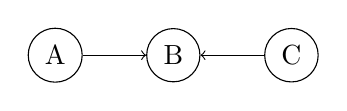
\begin{tikzpicture}[node distance=1.5cm]
        \tikzstyle{vertex}=[circle, draw, minimum size=0.6cm]
    
        \node[vertex] (A) {A};
        \node[vertex, right of=A] (B) {B};
        \node[vertex, right of=B] (C) {C};
        
        \draw[->] (A) -- (B);
        \draw[->] (C) -- (B);
    \end{tikzpicture}

\subsection{最小生成(代价)树, MST}

    包含连通图的全部顶点, 并且包含尽可能少的边. \textbf{边数 = 顶点数 - 1}. 最小生成树删去一条边变成非连通图; 新增一条边形成回路. 对于\textbf{带权连通无向图}, 生成树不同, 每棵树的权(\textbf{树中所有边的权之和})也可能不同. 仅无向图具有最小生成树. 最小生成树的权值之和最小

    当图中存在权重相同的边, 最小生成树可能不唯一; 当各边权值互不相等时, 最小生成树唯一.

    生成最小生成树的算法: Prim算法, Kruskal算法. 均使用贪心策略.

    \begin{lstlisting}[style = Pseudocode]
    GENERATE_MST (G) 
    {
        T = NULL;
        while (T 未形成MST) THEN
            寻找一条最小权重边 (u, v), 并且加入T后不会形成回路;
            T = T + (u, v);
        ENDWHILE
    }
    \end{lstlisting}

\newpage
\subsubsection{Prim算法}

    初始时任选一个顶点加入树, 在算法的每一轮过程中, 选择与当前树邻接, 且邻接边的权重最小的顶点, 将该顶点和边加入树, 直至生成树包含图的全部顶点.

    时间复杂度: $O(|V|^2)$. (在每一轮过程中, 搜索仍未加入树的结点, 选取权重最小的边. $(n-1) + (n-2) + \dots +1$). 不依赖于$|E|$, 适用于边稠密的图.

    % new two columns
    \begin{center}
    \begin{minipage}[t]{0.5\textwidth}
    \vspace{0pt}
        \begin{lstlisting}[style = Cpp]
            // Prim算法辅助结构
            struct MinEdge {
                int adjvex;    // 顶点
                EdgeType lowcost; // 最小权值
            };
        
            void MiniSpanTree_Prim(ALGraph& G, VertexType u) {
                MinEdge closedge[MaxVertexNum];
                int k = LocateVex(G, u);
                
                // 初始化closedge数组
                for (int j = 0; j < G.vexnum; j++) {
                    if (j != k) {
                        closedge[j].lowcost = INT_MAX;
                        closedge[j].adjvex = k;
                    }
                }
                
                // 处理起始顶点的邻接边
                ArcNode* p = G.vertices[k].firstarc;
                while (p != nullptr) {
                    int j = p->adjvex;
                    closedge[j].lowcost = p->weight;
                    closedge[j].adjvex = k;
                    p = p->nextarc;
                }
                
                closedge[k].lowcost = 0; // 将顶点u加入U集合
        \end{lstlisting}
    \end{minipage}
    \begin{minipage}[t]{0.45\textwidth}
    \vspace{0pt}
        \begin{lstlisting}[style=Cpp]
            cout << "Prim算法最小生成树边集:" << endl;
            // 选择其余G.vexnum-1个顶点
            for (int i = 1; i < G.vexnum; i++) {
                // 找出最小边
                int min = INT_MAX;
                int minIndex = -1;
                for (int j = 0; j < G.vexnum; j++) {
                    if (closedge[j].lowcost != 0 && closedge[j].lowcost < min) {
                        min = closedge[j].lowcost;
                        minIndex = j;
                    }
                }
                
                if (minIndex == -1) break;
                
                // 输出当前最小边
                cout << "边: " << G.vertices[closedge[minIndex].adjvex].data 
                    << " - " << G.vertices[minIndex].data 
                    << ", 权重: " << closedge[minIndex].lowcost << endl;
                
                // 将顶点minIndex加入U集合
                closedge[minIndex].lowcost = 0;
                
                // 更新closedge数组
                p = G.vertices[minIndex].firstarc;
                while (p != nullptr) {
                    int j = p->adjvex;
                    if (closedge[j].lowcost != 0 && p->weight < closedge[j].lowcost) {
                        closedge[j].lowcost = p->weight;
                        closedge[j].adjvex = minIndex;
                    }
                    p = p->nextarc;
                }
            }
        }
        \end{lstlisting}
    \end{minipage}
    \end{center}

\newpage
\subsubsection{Kruskal算法}

    初始时只有n个顶点没有边, 每个顶点都是一个连通分量. 按照边的权, 不断选择当前未被选取过且权最小的边, 若该边依附的两个顶点落在T中不同的连通分量上(边的两端未连通), 将该边加入树, 否则选择下一条权最小的边. 直至已经选取的边数达到$|V| - 1$.

    时间复杂度: 最坏情况需要对$|E|$都检查一次, 采用堆存储边集, 每次选择最小权值边需要$O(\log_2 |E|)$; 或对边做排序($O(|E| \log_2 |E|)$), 再使用并查集判断两个顶点是否属于同一个集合($O(\alpha(|V|))$, 增长极其缓慢, 视同常数). 总之, $T(n) = O(|E| \log_2 |E|)$, 不依赖$|V|$, 适合边稀疏而顶点多的图.

    % new two columns
    \begin{center}
    \begin{minipage}[t]{0.5\textwidth}
    \vspace{0pt}
        \begin{lstlisting}[style = Cpp]
            // Kruskal算法辅助结构
            struct Edge {
                int u, v;      // 边的两个顶点
                EdgeType weight; // 边的权重
                
                bool operator<(const Edge& other) const {
                    return weight < other.weight;
                }
            };
        
            // 并查集实现
            int Find(int parent[], int i) {
                while (parent[i] != -1) {
                    i = parent[i];
                }
                return i;
            }
        
            void Union(int parent[], int x, int y) {
                int xset = Find(parent, x);
                int yset = Find(parent, y);
                if (xset != yset) {
                    parent[xset] = yset;
                }
            }
                
            void MiniSpanTree_Kruskal(ALGraph& G) {
                vector<Edge> edges;
                
                // 收集所有边 (~只存储邻接矩阵的上三角)
                for (int i = 0; i < G.vexnum; i++) {
                    ArcNode* p = G.vertices[i].firstarc;
                    while (p != nullptr) {
                        // 避免重复添加无向图的边
                        if (i < p->adjvex) {
                            edges.push_back({i, p->adjvex, p->weight});
                        }
                        p = p->nextarc;
                    }
                }
        \end{lstlisting}
    \end{minipage}
    \begin{minipage}[t]{0.45\textwidth}
    \vspace{0pt}
        \begin{lstlisting}[style = Cpp]
            // 按权重排序
            sort(edges.begin(), edges.end());
            
            int parent[MaxVertexNum];
            for (int i = 0; i < G.vexnum; i++) {
                parent[i] = -1;
            }
            
            cout << "Kruskal算法最小生成树边集:" << endl;
            int count = 0; // 已选边数
            for (const Edge& e : edges) {
                if (count >= G.vexnum - 1) break;
                
                int root1 = Find(parent, e.u);
                int root2 = Find(parent, e.v);
                
                if (root1 != root2) {
                    cout << "边: " << G.vertices[e.u].data 
                        << " - " << G.vertices[e.v].data 
                        << ", 权重: " << e.weight << endl;
                    Union(parent, root1, root2);
                    count++;
                }
            }
        }
        \end{lstlisting}
    \end{minipage}
    \end{center}
    
\newpage
\subsection{最短路径}

    图是带权图时, 不能使用BFS. 最短路径分为: 单源最短路径(一个顶点到其他各个顶点的最短路径)和求每对顶点间的最短路径. 单源最短路径使用Dijkstra, 每对顶点间的最短路径使用Floyd, 在边权均非负时, 也可以轮流将每个顶点作为源点执行一个Dijkstra, $T(n) = O(|V| \cdot |V|^2) = O(|V|^3)$.

    \begin{center}
        \begin{tabular}{c|c|c|c}
            \toprule
             & BFS & Dijkstra & Floyd \\
            \midrule
            用途 & 单源最短路径 & 单源最短路径 & 各顶点之间距离 \\
            \midrule
            无权图 & 适用 & 适用 & 适用 \\
            \midrule
            带权图 & 不适用 & 适用 & 适用 \\
            \midrule
            带负权值 & 不适用 & 不适用 & 适用 \\
            \midrule
            \makecell{带负权回路 \\ (可能不存在最短路径)} & 不适用 & 不适用 & 不适用 \\
            \midrule
            时间复杂度 & $O(|V|^2)$ 或 $O(|V| + |E|)$ & $O(|V|^2)$ & $O(|V|^3)$ \\
            \bottomrule
        \end{tabular}       
    \end{center}


\subsubsection{Dijkstra}

    使用贪心算法, 时间复杂度为$O(|V|^2)$. 不适用于负权值图.

    使用三个辅助数组: \\
    \verb|final[]|: 标记各个顶点是否已经找到最短路径 \\
    \verb|dist[]|: 源点到其他顶点的当前的最短路径长度 \\
    \verb|path[]|: 源点到其他顶点的的最短路径上, 顶点i的前驱结点. \verb|path[0] = -1|

    \textbf{初始化} \verb|dist[]|: 对 \verb|path[i]|若源点$v_0$到$v_i$有弧, 这初始化为弧的权值, 否则为无穷

    \begin{lstlisting}[style = Pseudocode]
    // initial S
    S = {0};
    WHILE (V - S NOT empty) THEN
        select vj, dist[j] = min{dist[u] | u in V-S};
        S += j
        // update dist
        FOR k in V - S THEN
            dist[k] = min(dist[k], disk[j] + arcs[j][k])
        ENDFOR
    ENDWHILE
    \end{lstlisting}
    
    \newpage
    % new two columns
    \begin{center}
    \begin{minipage}[t]{0.5\textwidth}
    \vspace{0pt}
        \begin{lstlisting}[style = Cpp]
            // Dijkstra算法(邻接矩阵版本)
            void ShortestPath_Dijkstra_MG(MGgraph& G, VertexType v) 
            {
                DistInfo D[MaxVertexNum];
                int v0 = LocateVex_MG(G, v);
                
                if (v0 == -1) {
                    cout << "顶点不存在!" << endl;
                    return;
                }
                
                // 初始化
                for (int i = 0; i < G.vexnum; i++) {
                    D[i].dist = G.edge[v0][i];
                    D[i].visited = false;
                    if (D[i].dist < INF && i != v0) {
                        D[i].path = v0;
                    } else {
                        D[i].path = -1;
                    }
                }
                
                D[v0].dist = 0;
                D[v0].visited = true;
                
                // 主循环,每次求得v0到某个顶点v的最短路径
                for (int i = 1; i < G.vexnum; i++) {
                    EdgeType min = INF;
                    int minIndex = -1;
                    
                    // 选择当前未访问的最小距离顶点
                    for (int j = 0; j < G.vexnum; j++) {
                        if (!D[j].visited && D[j].dist < min) {
                            min = D[j].dist;
                            minIndex = j;
                        }
                    }
                    
                    if (minIndex == -1) break; // 剩余顶点不可达
                    
                    D[minIndex].visited = true;

                    // 更新通过minIndex到其他顶点的距离
                    for (int j = 0; j < G.vexnum; j++) {
                        if (!D[j].visited && G.edge[minIndex][j] < INF) {
                            if (D[minIndex].dist + G.edge[minIndex][j] < D[j].dist) {
                                D[j].dist = D[minIndex].dist + G.edge[minIndex][j];
                                D[j].path = minIndex;
                            }
                        }
                    }
                }
        \end{lstlisting}
    \end{minipage}
    \begin{minipage}[t]{0.45\textwidth}
    \vspace{0pt}
        \begin{lstlisting}[style = Cpp]
            // 输出结果
            cout << "Dijkstra算法结果(邻接矩阵)从顶点 " << v << " 到各顶点的最短路径:" << endl;
            for (int i = 0; i < G.vexnum; i++) {
                if (i != v0) {
                    cout << "到顶点 " << G.vex[i] << ": 距离=";
                    if (D[i].dist == INF) {
                        cout << "∞";
                    } else {
                        cout << D[i].dist;
                    }
                    cout << ", 路径: ";
                    
                    // 反向输出路径
                    vector<int> path;
                    int k = i;
                    while (k != -1) {
                        path.push_back(k);
                        k = D[k].path;
                    }
                    
                    for (int j = path.size() - 1; j >= 0; j--) {
                        cout << G.vex[path[j]];
                        if (j > 0) cout << " -> ";
                    }
                    cout << endl;
                }
            }
        }        
        \end{lstlisting}
    \end{minipage}
    \end{center}

    \newpage

    % new two columns
    \begin{center}
    \begin{minipage}[t]{0.45\textwidth}
    \vspace{0pt}
        \begin{lstlisting}[style = Cpp]
            // Dijkstra算法(邻接表版本)
            void ShortestPath_Dijkstra_AL(ALGraph& G, VertexType v) {
                DistInfo D[MaxVertexNum];
                int v0 = LocateVex_AL(G, v);
                
                if (v0 == -1) {
                    cout << "顶点不存在!" << endl;
                    return;
                }
                
                // 初始化距离数组
                for (int i = 0; i < G.vexnum; i++) {
                    D[i].dist = INF;
                    D[i].visited = false;
                    D[i].path = -1;
                }
                D[v0].dist = 0;
                
                // 使用优先队列优化(可选,这里使用简单实现)
                for (int i = 0; i < G.vexnum; i++) {
                    // 找到未访问的最小距离顶点
                    EdgeType min = INF;
                    int minIndex = -1;
                    for (int j = 0; j < G.vexnum; j++) {
                        if (!D[j].visited && D[j].dist < min) {
                            min = D[j].dist;
                            minIndex = j;
                        }
                    }
                    
                    if (minIndex == -1) break;
                    D[minIndex].visited = true;
                    
                    // 更新邻接顶点距离
                    ArcNode* p = G.vertices[minIndex].firstarc;
                    while (p != nullptr) {
                        int j = p->adjvex;
                        if (!D[j].visited && D[minIndex].dist + p->weight < D[j].dist) {
                            D[j].dist = D[minIndex].dist + p->weight;
                            D[j].path = minIndex;
                        }
                        p = p->nextarc;
                    }
                }
        \end{lstlisting}
    \end{minipage}
    \begin{minipage}[t]{0.5\textwidth}
    \vspace{0pt}
        \begin{lstlisting}[style = Cpp]
                // 输出结果
                cout << "Dijkstra算法结果(邻接表)从顶点 " << v << " 到各顶点的最短路径:" << endl;
                for (int i = 0; i < G.vexnum; i++) {
                    if (i != v0) {
                        cout << "到顶点 " << G.vertices[i].data << ": 距离=";
                        if (D[i].dist == INF) {
                            cout << "∞";
                        } else {
                            cout << D[i].dist;
                        }
                        cout << ", 路径: ";
                        
                        vector<int> path;
                        int k = i;
                        while (k != -1) {
                            path.push_back(k);
                            k = D[k].path;
                        }
                        
                        for (int j = path.size() - 1; j >= 0; j--) {
                            cout << G.vertices[path[j]].data;
                            if (j > 0) cout << " -> ";
                        }
                        cout << endl;
                    }
                }
            }
        \end{lstlisting}
    \end{minipage}
    \end{center}
    
\newpage
\subsubsection{Floyd}

    使用动态规划. 递推一个n阶的状态矩阵, $A^{(-1)}, A^{(0)}, \dots, A^{(n-1)}$. 每一轮允许新增一个顶点作为路径的中转点. 其中, $A^{(-1)}[i][j]$表示允许通过第k个顶点中转时, 顶点i到j的最短路径长度. 算法类似于矩阵链乘法的动态规划实现. 只能在邻接矩阵上实现(其他结构最终也需要构造出n阶矩阵), 适用于负权值图.
    \\
    时间复杂度: $O(|V| \dots |V|^2) = O(|V|^3)$, $|V|$轮, 每轮遍历$|V|^2$大小的矩阵. \\
    状态转移方程: 
    $
        A^{(k)}[i][j] = \min \{A^{(k-1)} [i][j], A^{(k-1)} [i][k] + A^{(k-1)} [k][j] \}, k=0, 1, \dots, n-1
    $ 
    \\
    初始化$A^{(-1)}[i][j] = arcs[i][j]$, 无<i, j>则初始化为无穷.
    \\
    回溯路径时, 查 \verb|path|, 若 \verb|path[i][j] = k|, 递归地查 \verb|path[i][k], path[k][j]| \\
    直至 \verb|path[i][k] == -1, path[k][j] == -1|
    
    % new two columns
    \begin{center}
    \begin{minipage}[t]{0.5\textwidth}
    \vspace{0pt}
        \begin{lstlisting}[style = Cpp]
            void ShortestPath_Floyd(MGgraph& G) {
                EdgeType A[MaxVertexNum][MaxVertexNum]; // 距离矩阵
                int path[MaxVertexNum][MaxVertexNum];   // 路径矩阵
                // 初始化
                for (int i = 0; i < G.vexnum; i++) {
                    for (int j = 0; j < G.vexnum; j++) {
                        A[i][j] = G.edge[i][j];
                        if (i != j && A[i][j] < INF) {
                            path[i][j] = i;
                        } else {
                            path[i][j] = -1;
                        } } }
                        
                // Floyd算法核心
                for (int k = 0; k < G.vexnum; k++) {
                    for (int i = 0; i < G.vexnum; i++) {
                        for (int j = 0; j < G.vexnum; j++) {
                            if (A[i][k] < INF && A[k][j] < INF && 
                                A[i][k] + A[k][j] < A[i][j]) {
                                A[i][j] = A[i][k] + A[k][j];
                                path[i][j] = path[k][j];
                            }
                        }
                    }
                }
                // 输出结果
                cout << "Floyd算法所有顶点对最短路径:" << endl;
                cout << "距离矩阵:" << endl;
                for (int i = 0; i < G.vexnum; i++) {
                    for (int j = 0; j < G.vexnum; j++) {
                        if (A[i][j] == INF) {
                            cout << setw(4) << "∞";
                        } else {
                            cout << setw(4) << A[i][j];
                        }
                    }
                    cout << endl;
                }
        \end{lstlisting}
    \end{minipage}
    \begin{minipage}[t]{0.45\textwidth}
    \vspace{0pt}
        \begin{lstlisting}[style = Cpp]
                // 输出具体路径
                cout << "\n具体路径:" << endl;
                for (int i = 0; i < G.vexnum; i++) {
                    for (int j = 0; j < G.vexnum; j++) {
                        if (i != j && A[i][j] < INF) {
                            cout << G.vex[i] << " 到 " << G.vex[j] << ": 距离=" << A[i][j] << ", 路径: ";
                            
                            vector<int> p;
                            int k = j;
                            while (k != i) {
                                p.push_back(k);
                                k = path[i][k];
                            }
                            p.push_back(i);
                            
                            for (int idx = p.size() - 1; idx >= 0; idx--) {
                                cout << G.vex[p[idx]];
                                if (idx > 0) cout << " -> ";
                            }
                            cout << endl;
                        } } } }
        \end{lstlisting}
    \end{minipage}
    \end{center}
    
    \begin{figure}[htbp]
        \centering
        \includegraphics[width=0.6\columnwidth]{dijkstra.png}
    \end{figure}

    \begin{figure}[htbp]
        \centering
        \includegraphics[width=0.8\columnwidth]{floyd.png}
    \end{figure}
    
    
    
    
\subsection{有向无环图(DAG)描述表达式}

    比如, 对于表达式 $((a + b) * (b * (c + d)) + (c + d) * e) * ((c + d) * e)$ 

    \begin{figure}[htbp]
        \centering
        \includegraphics[width=0.7\columnwidth]{DAG.png}
    \end{figure}

    \noindent
    1. 各操作数不重复地排成一排 \\
    2. 表达式按照运算顺序标出运算符符号 \\
    3. 依次加入运算符, 分层 (若需要利用下一层结果, 本运算符在上一层) \\
    4. 自底向上合并两侧操作数相同的运算符

    分层效果类似于 \\
    \verb|表达式: ((a + b) * (b * (c + d)) + (c + d) * e) * ((c + d) * e)| \\
    \verb|层次:       1    3    2    1     4    1    2    5     1    2|

\newpage
\subsection{拓扑排序}

    \textbf{顶点表示活动的网络(AOV网)}: 用有向无环图表示一个工程, 顶点表示活动, 弧$<V_i, V_j>$表示活动$V_i$必须先于$V_j$进行. AOV网是有向无环图. 

    \textbf{拓扑排序}: 由一个有向无环图的顶点组成的序列, 且满足以下条件 \\
    (1) 每个顶点均出现且只出现一次; \\
    (2) 若顶点A在序列中排在B之前, 这图中不存在从B到A的路径

    \begin{lstlisting}[style = Pseudocode]
    Function 拓扑排序 (Graph G) {
        WHILE (G NOT empty || G 无入度为0的顶点) THEN
            select v ( ID(v) = 0(无前驱) ) ;
            delete v and all <v, x>;
        ENDWHILE
    }
    \end{lstlisting}

    时间复杂度: 邻接表$O(|V| + |E|)$; 邻接矩阵: $O(|V|^2)$

    \begin{lstlisting}[style = Pseudocode]
        Function 逆拓扑排序 (Graph G) {
            WHILE (G NOT empty || G 无出度为0的顶点) THEN
                select v ( OD(v) = 0(无后继) ) ;
                delete v and all <x, v>;
            ENDWHILE
        }
    \end{lstlisting}

    \noindent
    逆拓扑排序: 可以选择逆邻接表(边表存储的是指向结点的边) \\
    \textbf{拓扑排序与环的关系}: 在拓扑排序中, 若网中不存在ID=0的顶点, 则必然存在环.
    
    \begin{figure}[htbp]
        \centering
        \includegraphics[width=0.7\columnwidth]{sort.png}
    \end{figure}

    \noindent
    拓扑排序的结果可能不唯一; AOV网必定有拓扑排序, 但是存在拓扑排序的图不一定是AOV网 \\
    判断拓扑排序是否唯一的判断条件是: 每次输出顶点式, 检测入度为0的顶点数目是否为1, 若每次都唯一, 则拓扑排序序列唯一 \\
    AOV网中每个顶点的编号是人为指定的, 可以按照排序序列依次重新编号生成新的AOV邻接存储矩阵, 可以将原先的矩阵转换为\textbf{三角矩阵}以压缩存储; 若一个的邻接矩阵是三角矩阵, 则必定存在拓扑序列, 反之不一定成立
    
    \newpage

    % new two columns
    \begin{center}
    \begin{minipage}[t]{0.5\textwidth}
    \vspace{0pt}
    \begin{lstlisting}[style = Cpp]
        // 邻接矩阵拓扑排序(Kahn算法 - 基于入度)
        bool TopologicalSort_MG_Kahn(MGgraph& G) {
            vector<int> inDegree(G.vexnum, 0);
            queue<int> q;
            vector<VertexType> result;
            
            // 计算每个顶点的入度
            for (int i = 0; i < G.vexnum; i++) {
                for (int j = 0; j < G.vexnum; j++) {
                    if (G.edge[i][j] != 0) {
                        inDegree[j]++;
                    }
                }
            }
            
            // 将入度为0的顶点加入队列
            for (int i = 0; i < G.vexnum; i++) {
                if (inDegree[i] == 0) {
                    q.push(i);
                }
            }
            
            int count = 0; // 记录已输出的顶点数
            while (!q.empty()) {
                int v = q.front();
                q.pop();
                result.push_back(G.vex[v]); // 存入用于输出的vector
                count++;
                
                // 减少所有邻接顶点的入度
                for (int i = 0; i < G.vexnum; i++) {
                    if (G.edge[v][i] != 0) { // <v, i>
                        inDegree[i]--;
                        if (inDegree[i] == 0) { // 新的无前驱结点
                            q.push(i);
                        }
                    }
                }
            }
            
            // 若可以拓扑排序, 则全部结点应该已经存入result
            if (count != G.vexnum) { 
                cout << "图中存在环,无法进行拓扑排序!" << endl;
                return false;
            }
            
            cout << "拓扑排序结果(Kahn-邻接矩阵): ";
            for (VertexType v : result) {
                cout << v << " ";
            }
            cout << endl;
            return true;
        }
    \end{lstlisting}
    \end{minipage}
    \begin{minipage}[t]{0.45\textwidth}
    \vspace{0pt}
    若使用邻接表, 则需要改动入度计算和改变入度的逻辑
    
    \begin{lstlisting}[style = Cpp]
        // 计算每个顶点的入度
        for (int i = 0; i < G.vexnum; i++) {
            ArcNode* p = G.vertices[i].firstarc;
            while (p != nullptr) {
                inDegree[p->adjvex]++;
                p = p->nextarc;
            }
        }
        // 减少所有邻接顶点的入度
        ArcNode* p = G.vertices[v].firstarc;
        while (p != nullptr) {
            int adjvex = p->adjvex;
            inDegree[adjvex]--;
            if (inDegree[adjvex] == 0) {
                q.push(adjvex);
            }
            p = p->nextarc;
        }
    \end{lstlisting}

    若需要逆拓扑排序, 逆向输出result. 或者拓扑使用队列, 逆拓扑使用栈

    \end{minipage}
    \end{center}
    
    \begin{center}
    \begin{minipage}[t]{0.5\textwidth}
    \vspace{0pt}
        \textbf{DFS实现拓扑排序的思路}

        \vspace{-0.5\baselineskip}
        \begin{verbatim}
对每个未访问的结点执行DFS 
标记当前结点为正在访问 
访问每个邻接点 
    如果邻居为正在访问, 有环, 报错 
    如果邻居为访问完, 跳过 
    如果邻居为未访问, 递归DFS 
标记当前结点为未访问 
标记当前结点为访问完 
当前结点压入结果序列头部, 退栈
        \end{verbatim}

        \vspace{-1.5\baselineskip}
        \textbf{逆拓扑排序}只需要逆转拓扑序列, \\
        或者拓扑用栈, 逆拓扑用队列
        
        \noindent
        \verb|visited[]|: \\
        判断顶点是否已在拓扑序列中, 阻止重复排序 \\
        \verb|visiting[]|: \\
        判断顶点是否在当前DFS搜索路径上, 检测环, \\
        阻止无限递归

        \indent\par
        \textbf{为什么需要两个辅助数组}: 考虑图

        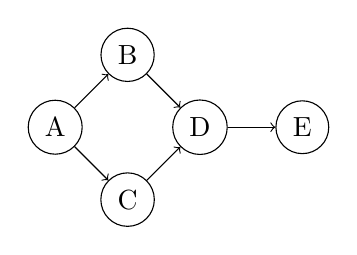
\begin{tikzpicture}[node distance=1.3cm]
            \tikzstyle{vertex}=[circle, draw, minimum size=0.3cm]
        
            \node[vertex] (A) {A};
            \node[vertex, above right of=A] (B) {B};
            \node[vertex, below right of=A] (C) {C};
            \node[vertex, below right of=B] (D) {D};
            \node[vertex, right of=D] (E) {E};
            
            \draw[->] (A) -- (B);
            \draw[->] (A) -- (C);
            \draw[->] (C) -- (D);
            \draw[->] (B) -- (D);
            \draw[->] (D) -- (E);
        \end{tikzpicture}

        \noindent
        简记 \verb|visited[i]=a, visiting[i]=b| 为i:(a, b) \\
        排序过程为: \\
        access A, A:(false, true); access B, B:(false, true); \\
        access D, D:(false, true); access E, E:(false, true); \\
        return to A. \\
        A:(false, true); B:(true, false) \\
        D:(true, false); E:(true, false) \\
        access C, C(false, true); return to A \\
        >> Topo: ACBDE

        若只设置visited[], visited[i]=a简记为: i:(a) \\
        access A, A:(true); access B, B:(true) \\
        access D, D:(true); access E, E:(true) \\
        return to A \\
        A:(true), B(false), D(false), E(false) \\
        access C, C:(true); access D, D:(true); access E, E:(true)\\
        拓扑结果[C, D, E, B, D, E] \\
        至此, 可以看见只设置一个数组时, \\
        随着退栈时visited状态复原为false, \\
        一个结点可能会被计入两条拓扑序列中, 显然错误. \\
        若不还原, DFS无法进行

    \end{minipage}
    \begin{minipage}[t]{0.45\textwidth}
    \vspace{0pt}
    \begin{lstlisting}[style = Cpp]
        // Topo递归部分
        bool DFS_Topo(ALGraph &G, int v,
                    vector<bool> &visiting,
                    vector<bool> &visited,
                    stack<int> &S)
        {
            visiting[v] = true;

            for (ArcNode *p = G.vertices[v].firstarc; p != nullptr; p = p->nextarc) {
                int w = p->adjvex;

                if (visiting[w]) {
                    // 回到递归栈 — 必有环
                    return false;
                }

                if (!visited[w]) {
                    if (!DFS_Topo(G, w, visiting, visited, S))
                        return false;
                }
            }

            visiting[v] = false;  // 离开递归栈
            visited[v] = true;    // 已完成
            S.push(v);
            return true;
        }
        // Topo主过程
        bool TopoSort_DFS(ALGraph &G)
        {
            vector<bool> visiting(G.vexnum, false);
            vector<bool> visited(G.vexnum, false);

            stack<int> S;

            for (int i = 0; i < G.vexnum; i++) {
                if (!visited[i]) {
                    if (!DFS_Topo(G, i, visiting, visited, S)) {
                        cout << "Graph has a cycle. Topological sort impossible." << endl;
                        return false;
                    }
                }
            }

            cout << "Topo Order (DFS): ";
            while (!S.empty()) {
                cout << G.vertices[S.top()].data << " ";
                S.pop();
            }
            cout << endl;
            return true;
        }
    \end{lstlisting}
    \end{minipage}
    \end{center}

\newpage
\subsection{关键路径}
    
    \textbf{AOE网}: 用边表示活动的网络. 带权有向图, 顶点表示事件, 有向边表示活动, 边的权值表示完成该活动的开销. AOE网是有向无环图. \textbf{源点(开始顶点)}: 仅有的1个入度为0的顶点; \textbf{汇点(结束顶点)}: 仅有的一个出度为0的顶点. AOE网中, 有些活动可以并行进行. \textbf{关键路径}: 具有最大路径长度的路径, \textbf{关键活动}: 关键路径上的活动. \textbf{完成整个工程的最短时间}: 关键路径的长度.

    \begin{center}
    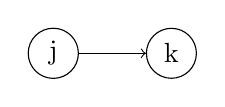
\begin{tikzpicture}[node distance=1.5cm]
        \tikzstyle{vertex}=[circle, draw, minimum size=0.6cm]
    
        \node[vertex] (A) {j};
        \node[vertex, right of=A] (B) {k};
        
        \draw[->] (A) -- (B);
    \end{tikzpicture}
    \end{center}

    \noindent
    事件的\textbf{最早发生时间}$v_e (k)$: $v_e(\mbox{源点}) = 0$; $v_e(k) = \max \{v_e(j) + weight<j, k>\}$ \\
    事件的\textbf{最迟发生时间}$v_l(k)$: $v_l(\mbox{汇点}) = v_e(\mbox{汇点})$; $v_l(j) = \min \{v_l(k) - weight<j, k>\}$ \\
    活动的\textbf{最早开始时间}$e(i)$: $<j, k>$表示活动$a_i$, 则$e(i) = v_e(j)$ (弧尾事件的最早发生时间) )\\
    活动的\textbf{最迟开始时间}$l(i)$: $<j, k>$表示活动$a_i$, 则$l(i) = v_l(k) - weight<j, k>$ (弧头最迟发生时间 - 开销) \\
    活动最迟开始时间与最早开始时间的差额: $d(i) = l(i) - e(i)$, 该活动的\textbf{时间余量或可以拖延的时间}, $d(i) = 0$的活动为关键活动.

    \textbf{求关键路径的算法}

    \vspace{-1\baselineskip}
    \begin{verbatim}
1. 从源点出发, 令其ve=0, 按拓扑序列求其余顶点最早发生时间
2. 从汇点出发, 令其vl=ve, 按逆拓扑排序序列求其余顶点最迟发生时间
3. 求各弧的e(), l()
4. 求各个活动的d(), 找出全部d=0的活动
    \end{verbatim}
    
    \vspace{-1.5\baselineskip}
    \noindent
    1. 加快关键活动可以缩短整个工程的工期, 但是不能任意缩短, 缩短到一定程度, 关键活动会变成非关键活动 \\
    2. 对于有几条关键路径的网, 只提高一条关键路径上的关键活动速度不能缩短工期, 必须加快包含在所有关键路径上的关键活动才能缩短工期
    
    \begin{figure}[htbp]
        \centering
        \includegraphics[width=0.55\columnwidth]{event1.png}
    \end{figure}
    
    \begin{figure}[htbp]
        \centering
        \includegraphics[width=0.6\columnwidth]{event2.png}
    \end{figure}
    
    \textbf{快速求出关键路径}
        
    \noindent
    只需要求出$v_e$, 在每次取max中, 舍弃产生较小值的边. $v_e(1) = 0; v_e(2) = 3; v_e(3) = 2;$ \\
    $v_e(4) = \max \{v_e(2) + 2, v_e(3) + 4\} \max \{5, 6\} = 6, \mbox{舍弃}a_3; $ \\
    $v_e(5) = v_e(2) + 3 = 6; $ \\$
    v_e(6) = \max \{v_e(5) + 1, v_e(4) + 2, v_e(3) + 3\} = \max \{7, 8, 5\} = 8, \mbox{舍弃} a_8, a_6$. \\
    剩下的边里面, 从源点到汇点的只有$a_2 -> a_5 -> a_7$

    
    
    

    


    
    
    



\end{sloppy}
\end{document}